\chapter{Avaliação exploratória}

\section{Cenário-tipo selecionado}

%explicar qual foi o cenário selecionado para experimentar em cada plataforma (deve ser uma parte dos requisitos gerais do capítulo 3)
Antes de avançar com o desenvolvimento do sistema foi necessário escolher um backend para dar suporte tanto à aplicação móvel, como à aplicação web. Para isso foi desenvolvido um cenário idêntico com ambos os backends em que pudéssemos fazer uma análise comparativa dos pontos fortes e ou fracos entre eles. \par 
O cenário escolhido para esta avaliação exploratória foi o simples ato de recolher a frequência cardíaca do sensor do \gls{VJ} e guardar no backend em estudo, para posteriormente visualizar um simples histórico dos dados inseridos. Na figura \ref{f:study-overview} temos uma simples visão das várias partes envolvidas nesta avaliação.

\begin{figure}[H]
  \centering
  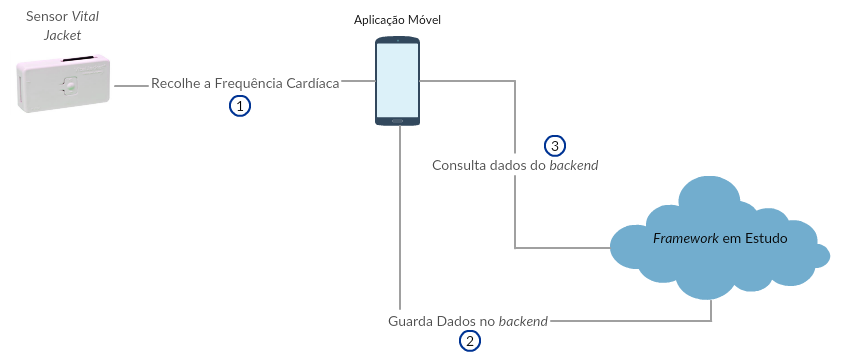
\includegraphics[width=0.9\textwidth]{imgs/study-overview.png}
  \caption[Diagrama geral do cenário de estudo]{Diagrama geral do cenário de estudo}
  
  \label{f:study-overview}
\end{figure}

A escolha de um backend para a solução era um ponto importante. Das várias frameworks disponíveis para um possível backend foram selecionadas três para ser desenvolvido o cenário com o objetivo de concluir se seria uma boa hipótese para a solução, entre elas estão: \gls{OMH}, \gls{FHIR} e Google Fit. \par

Para utilizar cada uma destas frameworks, foi desenvolvida uma aplicação móvel, bastante simples, a aplicação móvel tinha várias funcionalidades. Entre elas temos:
\begin{itemize}
  \item Seleccionar o dispositivo com os sensores
  \item Efetuar Login na respetiva framework
  \item Guardar leituras de frequência cardíaca num determinado segundo
  \item Visualizar as leituras inseridas
\end{itemize}

Tendo em conta que a mesma aplicação conseguia utilizar os três backends distintos, esta seleção era feita tendo em conta o tipo de login efetuado.

\clearpage

\section{Implementação exploratória: Open mHealth}
%http://www.openmhealth.org/documentation/#/store-data/storage-overview
%http://projects.spring.io/spring-security-oauth/docs/oauth2.html
%explicar a implementação que foi feita para esta tecnologia, dificuldades, adaptações, "gaps"


Relativamente a este backend para solução do problema proposto temos à nossa disponibilidade um serviço denominado de \gls{DSU} que disponibiliza uma \gls{API} \gls{REST} denominada de ''dataPoint API''. A \gls{API} suporta a criação, consulta e eliminação de dados. Esta \gls{API} permite a autorização utilizando o protocolo de autorização OAuth 2.0. Em suma este serviço é composto por um servidor de dados e um servidor de autorização. O servidor de autorização gere a concessão de tokens de acesso. \cite{omhstorage} \par
Com a introdução desta peça para o estudo exploratório ficamos com uma arquitetura que está representada na figura \ref{f:exp-omh-arch}.

\begin{figure}[H]
  \centering
  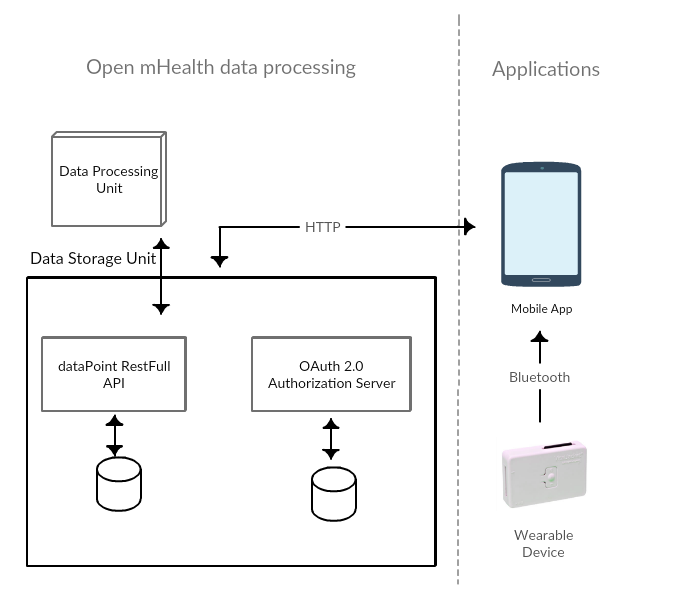
\includegraphics[width=0.9\textwidth]{imgs/omh-arch-exp.png}
  \caption[Arquitetura do caso exploratório com o Open mHealth]{Arquitetura do caso exploratório com o Open mHealth}
  
  \label{f:exp-omh-arch}
\end{figure}

\subsection{Implementação adicional}

Foi adicionado ao processo de inserção dos denominados ''dataPoint'' que é um documento que representa e deve estar em conformidade com um dos tipos de dados disponíveis denominados ''dataschemas''. Apesar dos ''dataschemas'' especificarem um formato de dados, esta validação relativa ao formato de dados não estava a ser efetuada. Um ''datapoint'' é composto por um cabeçalho onde também é definido o tipo de dados associado, e por um corpo que é formatado através do ''dataschema'' associado. Foi então feita esta validação adicional, quando o datapoint chega para ser guardado, é validado para verificar se está formatado convenientemente. Esta validação é importante para posteriores consultas e tratamentos dos dados de maneira igual para cada tipo.
\par 


A \gls{OMH} tem definido um conjunto de ''data schemas'' \cite{omhschemas} que é um conjunto de esquemas de dados criados e disponíveis que especificam um formato de dados para um determinado conteúdo como por exemplo a frequência cardíaca\cite{omhschemas}. Este conjunto de schemas pode ser estendido. Ao criar um novo tipo de dados(um novo ''data schema'') podemos reutilizar outros já existentes, criando um ''data schema'' que mesmo não sendo normalizado, utiliza para definição de determinadas propriedades outros ''data schemas'' normalizados. Para experimentar esta funcionalidade foi então adicionado um novo esquema de dados para que o sistema conseguisse suportar \gls{ECG}. Esta experimentação foi conseguida com sucesso e foi uma coisa que saiu um pouco fora do cenário objetivo mas serviu para conseguir perceber muito melhor a framework. \par 
As dificuldades encontradas não foram muitas, pois a framework estava bastante bem estruturada e o grau de complexidade era aceitável. As possíveis falhas desta framework era a falta de esquemas de dados para o acelerómetro, \gls{ECG} e para dados demográficos dos utilizadores da framework.
\clearpage

\section{Implementação exploratória: FHIR}
%http://hapifhir.io/doc_jpa.html

\begin{figure}[H]
  \centering
  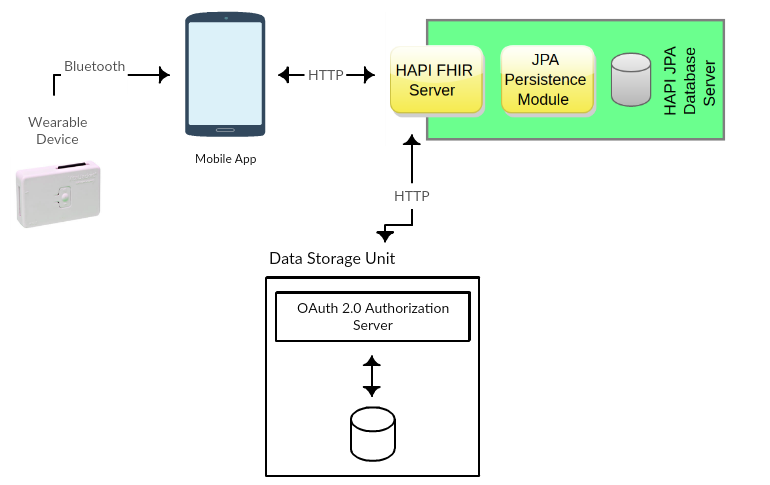
\includegraphics[width=0.9\textwidth]{imgs/fhir-arch-exp.png}
  \caption[Arquitetura do caso exploratório com o FHIR]{Arquitetura do caso exploratório com o FHIR}
  
  \label{f:exp-fhir-arch}
\end{figure}

\clearpage


\section{Implementação exploratória: Google Fit}
%https://developers.google.com/fit/rest/

\section{Resultados e lições aprendidas}
\textcolor{red}{{\huge TODO}}//todo
%ico: sistematizar aquilo que foi possível concluir das implementações exploratórias discutir pontos forte / fracos observados

\cleardoublepage